
\begin{frame}
  \frametitle{Helpful remarks}
  scheduling a task at $\bmax$ during $\inter$ gives the higher energy amount ($f_i$ is non decreasing)
  \begin{center}
    \begin{tikzpicture}
      [yscale=0.6]
      [inner sep=0]
      \node (O) at (0,0) {};
      \node (T) [right of=O,node distance=4cm] {};
      \node (t1) [right of =O, node distance=1cm] {};
      \node (t2) [right of =t1, node distance=2cm] {};
      \draw[pattern=north west lines] (t1) rectangle (3,2.5);
      \draw[dashed,gray!40!] (0,2.5) -- (4,2.5) node[right] {$\bmax$};
      
      \draw[red,dashed] (t1) node[below] {$t_1$}-- (1,3);
      \draw[red,dashed] (t2) node[below] {$t_2$} -- (3,3);
      \draw[->] (O) -- (T);
    \end{tikzpicture}
  \end{center}
  
  \begin{block}{Notations}
    \begin{itemize}
    \item the latest start time of $i$ as $\smax=d_i-\frac{W_i}{f_i(\bmax)}$
    \item and the earliest end time of $i$ as $\emin=r_i+\frac{W_i}{f_i(\bmax)}$
    \end{itemize}
  \end{block}
  $\Rightarrow$ a task can start in $\inter[r_i][\smax]$ and end in $\inter[\emin][d_i]$
\end{frame}

\begin{frame}
  \frametitle{Trick for the MILP formulation}
  \textbf{Question:} How formulate a continuous problem with a MILP?
  
  \begin{theorem}
    Any solution can be transformed in a solution where $\forall i \in A,\ b_i(t)$ is piecewise constant. 
  \end{theorem}
  \begin{proof}[Proof (Sketch)]
    \begin{columns}
      \begin{column}{0.55\linewidth}
        \begin{overlayarea}{\textwidth}{5cm}
          \only<1-8>{            
            \begin{itemize}
            \item<3-> $(t_q)$: series of start and end times
              \vspace{0.2cm}
            \item<4-> in $\inter[t_q][t_{q+1}]$, $b'_i(t)$ is set to the mean value of $b_i(t)$ over this interval
              \vspace{0.4cm}
            \item<8-> same resource and energy amount
              \vspace{0.4cm}
            \end{itemize}
            
          }
          \only<9>{
            \vspace{1cm}
            \centering 
            {\bf Remark: }we have only to \\
            change at $st_i$ or $ft_i$ \\
            \vspace{0.5cm}
            = ``events''
          }
        \end{overlayarea}
      \end{column}
      \begin{column}{0.45\linewidth}
        \onslide<2->{
          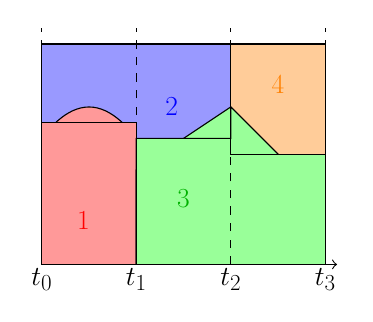
\begin{tikzpicture}
            [scale=0.4,transform shape]
            [inner sep =0]
            \node (O) at (0,0) {};
            \node (T) [right of=O,node distance=9.5cm] {};
            
            \fill[blue!40!,draw=black] (0,3) rectangle (6,7) node[midway, right=0.8cm] {\color{blue} \Huge $2$};
            \onslide<2-4>{
              \fill[red!40!,draw=black] (0,0) node[above right=1cm] {\color{red} \Huge$1$}-- (0,4) parabola bend (1.5,5) (3,4) --(3,0) -- cycle;}
            \onslide<5->{
              \fill[red!40!,draw=black] (0,0) node[above right=1cm] {\color{red} \Huge$1$}-- (0,4.5) --(3,4.5) --(3,0) -- cycle;}
            \fill[orange!40!,draw=black] (9,7) rectangle (6,2) node[midway, above= 0.8cm] {\color{orange} \Huge $4$};
            \onslide<2-5>{
              \fill[green!40!,draw=black] (3,0) -- (9,0) -- (9,2) -- (6,5)-- (3,3)  node[below, right=2cm] {\color{black!30!green} \Huge $3$}-- cycle;}
            \onslide<6>{
              \fill[green!40!,draw=black] (3,0) -- (9,0) -- (9,2) -- (6,5)-- (6,4)  node[left=1.5cm,below=1.5cm] {\color{black!30!green} \Huge $3$} --(3,4) -- cycle;
            };
            \onslide<7->{
              \fill[green!40!,draw=black] (3,0) -- (9,0) -- (9,3.5) -- (6,3.5)-- (6,4)  node[left=1.5cm,below=1.5cm] {\color{black!30!green} \Huge $3$} --(3,4) -- cycle;
            };
            \draw[->] (O) -- (T);
            \onslide<3->{
              \draw[dashed] (0,0) node[below] {\Huge $t_0$} -- (0,7.5);
              \draw[dashed] (3,0) node[below] {\Huge $t_1$} -- (3,7.5);
              \draw[dashed] (6,0) node[below] {\Huge $t_2$} -- (6,7.5);
              \draw[dashed] (9,0) node[below] {\Huge $t_3$} -- (9,7.5);
            }
          \end{tikzpicture}
        }
      \end{column}
    \end{columns}
\vspace{-1cm}
  \end{proof}
\end{frame}

